After obtaining the necessary parameters for the proposed model, we quantitatively and qualitatively evaluate its prediction performance on 8 distorted videos in the testing set. Alternatively, the discussion on the results is also performed.

To quantitatively assess the prediction performance, the correlation between the subjective overall QoE obtained in the LFOVIA Video QoE Database \cite{LFOVIA} and our predicted cumulative QoE at the end of each video was computed. It is crucial to note that the subjective overall QoE can be considered as the cumulative perception of the user at the end of streaming session. There were three evaluation metrics utilized for evaluation: 1) Pearson Correlation Coefficient (PCC), 2) Spearman Rank Order Correlation Coefficient (SROCC), and 3) Root Mean Square Error (RMSE). Typically, PCC and SROCC quantify how well the predicted QoE tracks the actual QoE scores in the database, whereas, RMSE indicates the closeness between them. We also compared our proposed model with a reference method of \cite{CumulativeQoE_Assessing}, using the same training set and testing set. The cumulative QoE model in \cite{CumulativeQoE_Assessing} is characterized by the following equation: 

\begin{equation}
    Q_{t} = \gamma Q_{t-1} + (1-\gamma)q_{t}
\end{equation}

where $q_{t}$ is the instantaneous user experience at moment $t$, $Q_{t-1}$ is the cumulative QoE at the previous moment $t-1$, and $\gamma$ is the memory strength parameter. The correlation between the predicted cumulative QoE obtained from this model and the subjective overall QoE in LFOVIA database was also investigated through PCC, SROCC and RMSE metrics. We reported the performance of our model and the reference method in Table \ref{tbl:PerformanceDataset}. This result shows a superior prediction performance of our model. Figure \ref{fig:PCC_CumulativeQoe_OverallQoE} additionally emphasizes the competitive performance of our model. Thereby, the proposed model has effectively assessed cumulative perception over multiple scenarios in testing videos. 

% \begin{table}[tb]
%   
%   \centering
%   \begin{tabular}{cccc}
%     \toprule
%     & $\textbf{PCC}$ & $\textbf{SROCC}$ & $\textbf{RMSE}$\\
%     \midrule
%     \cite{CumulativeQoE_Assessing} & 0.4292 & 0.4048 & 7.931 \\
%     Proposed Model & \textbf{0.7664} & \textbf{0.7857} & \textbf{4.654} \\
%     \bottomrule
%   \end{tabular}
%   \label{tbl:PerformanceDataset}
% \end{table}

\begin{table}[tb]
\caption{Prediction performance of the reference model and our proposed model over training and testing set}
\centering
\begin{tabular}{|l|l|c|c|c|}
\hline
& & PCC & SROCC & RMSE \\
\hline
\multicolumn{1}{|l|}{\multirow{2}{*}{Training}}   & \multicolumn{1}{l|}{\cite{CumulativeQoE_Assessing}}                  & 0.7413       & 0.6420         & 10.6187        \\
\multicolumn{1}{|l|}{}                                & \multicolumn{1}{l|}{Proposed model}  & \textbf{0.9441}       & \textbf{0.8604}         & \textbf{4.1525}         \\
\hline
\multicolumn{1}{|l|}{\multirow{2}{*}{Testing}}    & \multicolumn{1}{l|}{\cite{CumulativeQoE_Assessing}}                  & 0.2777       & 0.2381         & 7.5135         \\
\multicolumn{1}{|l|}{}                                & \multicolumn{1}{l|}{Proposed model}  & \textbf{0.7664}       & \textbf{0.7857}         & \textbf{4.6538}         \\
\hline
\end{tabular} \label{tbl:PerformanceDataset}
\end{table}


\begin{figure}[tb]
  \centering
  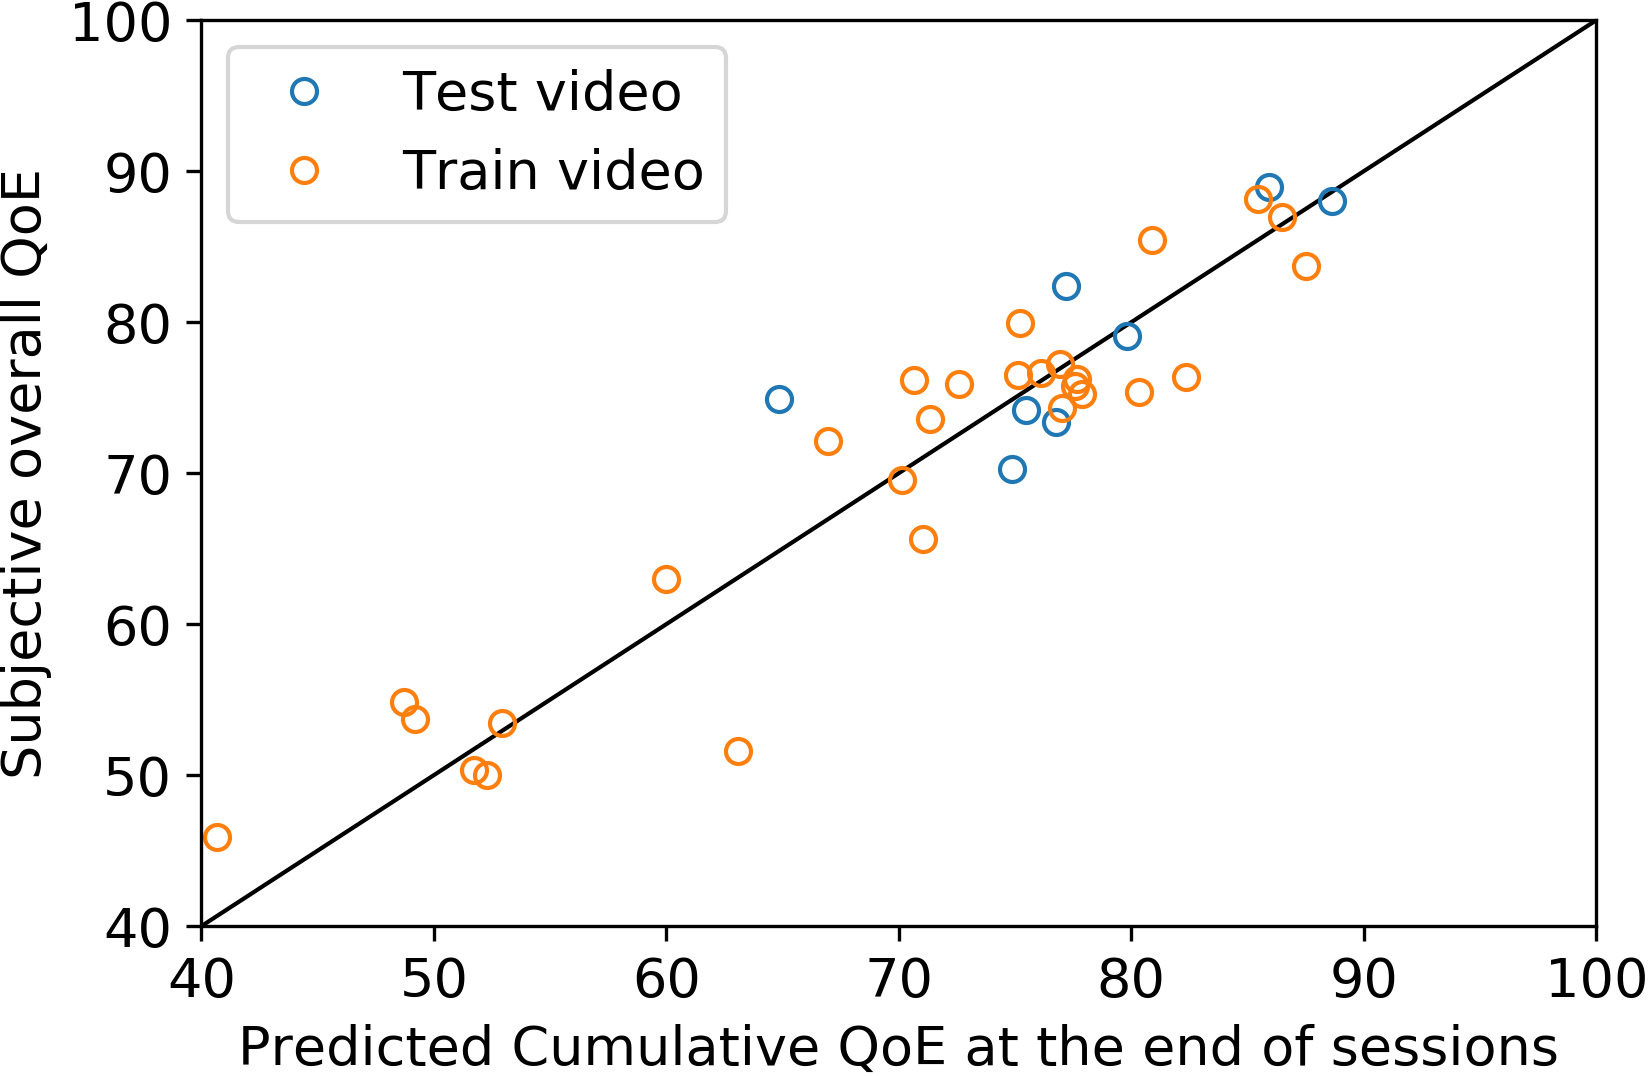
\includegraphics[width=0.5\linewidth]{\FigsDir/pcc_cmqoe_overallqoe.png}
  \caption{Correlation between subjective overall QoE and predicted cumulative QoE at the end of streaming session}
  \label{fig:PCC_CumulativeQoe_OverallQoE}
\end{figure}

\begin{figure}[tb]
  \centering
  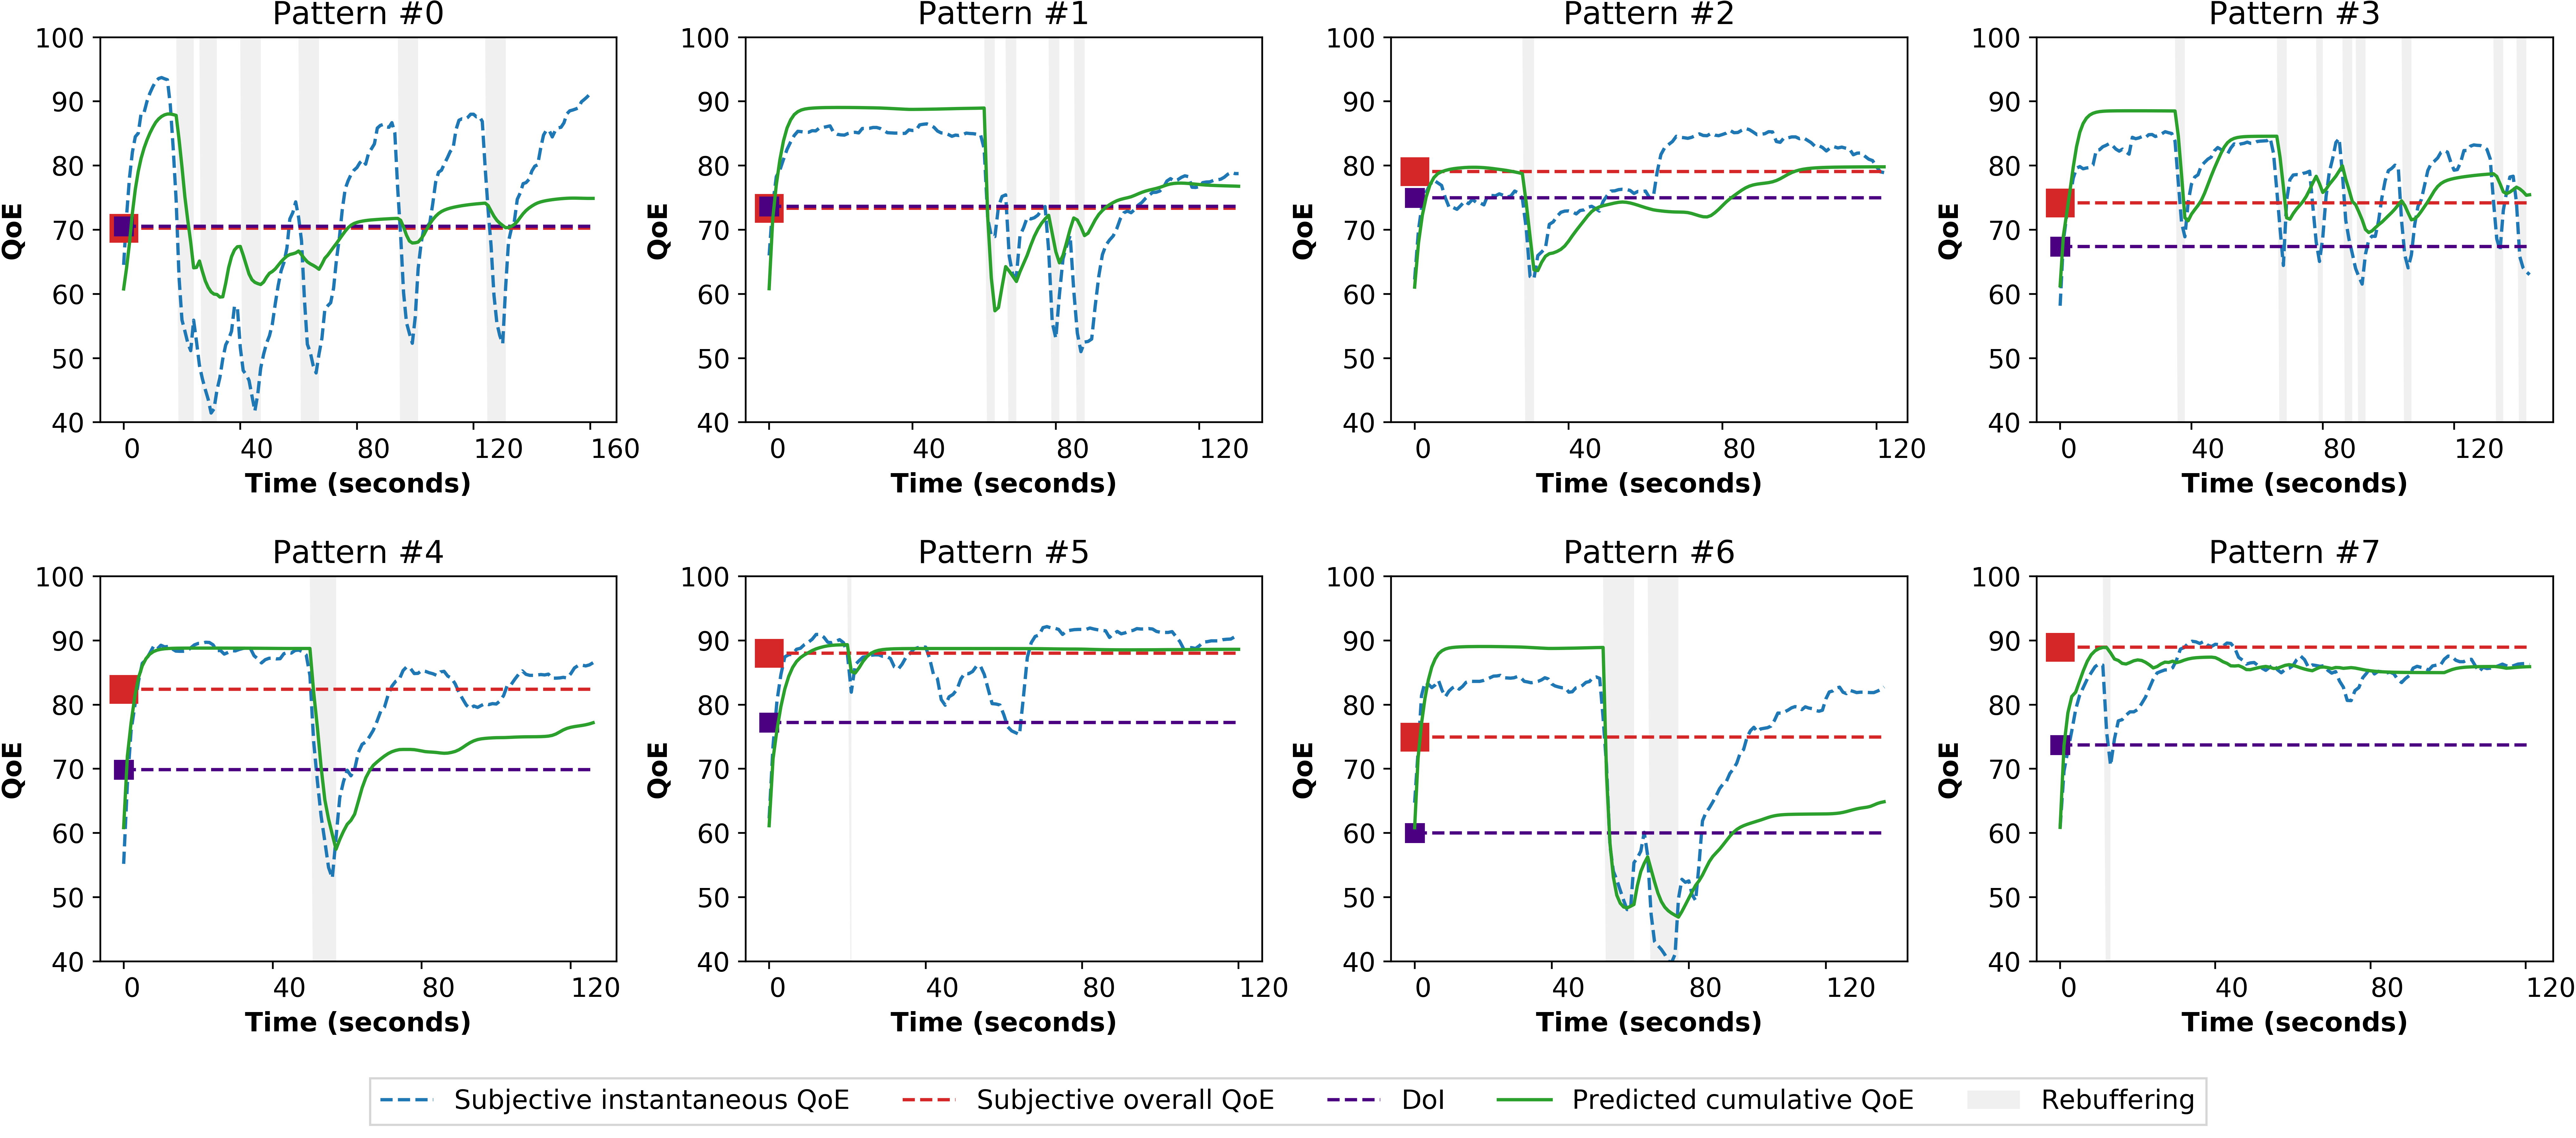
\includegraphics[width=\linewidth]{\FigsDir/cumulative_performance_dataset.png}
  \caption{Predicted cumulative QoE in comparison with the subjective overall and instantaneous QoE over eight different playout patterns}
  \label{fig:Cumulative_Performance}
\end{figure}


In qualitative evaluation, our purpose is to validate the impact of memory effects and DoI on the cumulative QoE prediction over multiple scenarios on testing videos. Thereby, the prediction performance of the proposed model in a short period and longer period can be assessed. For that reason, in Figure \ref{fig:Cumulative_Performance}, we plot the predicted cumulative QoE in comparison with both subjective instantaneous QoE and subjective overall QoE which are obtained from the database. From now, the terms of subjective instantaneous QoE and subjective overall QoE will be referred to as instantaneous QoE and overall QoE for short. 

In general, the predicted cumulative QoE precisely reacts to any interruption at any moment while being close to the overall QoE at the end of the streaming session. For the initial interruption, it is always witnessed a significant deterioration in predicted cumulative QoE. Nevertheless, when such unpleasant events continuously occur, the predicted cumulative QoE tends to decrease at a lower rate. Additionally, a lower recovering rate is subsequently introduced after each event. 

%/=======================================
\subsubsection{Impacts of memory effects}

  In pattern \#2, \#5, \#7, there is only one interruption with short duration occurring near the beginning of streaming sessions. As a result, the predicted cumulative QoE introduces a slight decrease, following by a gradual recovery and convergences at the values as close to the overall QoE. These trends are consistent with those of instantaneous QoE. It means that the prediction accurately demonstrates the role of forgetting curve characteristic as well as the recency effect. More concretely, after the finishing of the interruption, the memory intensity about such event starts to exponentially decay, leading to the recovery in perceived video quality. At the end of streaming sessions, there is a possibility that the decay has completely finished, in other words, the memory of distorted events is vanished. Therefore, the recency effect becomes dominant, leading to the consistency among the predicted cumulative QoE, instantaneous QoE, and overall QoE.
  
  In pattern \#0 and \#1, rebuffering event repeatedly occurs in the middle of streaming sessions. While the predicted cumulative QoE is consistent with the overall QoE at the end of sessions, the instantaneous QoE tends to continuously increase, creating a big gap to the overall QoE. At first sight, one might think that the overall QoE must be as high as the instantaneous QoE at the end of streaming sessions due to the recency effect. This inference is understandable because the moment at which the last interruption occurs is quite far from the end of sessions, thus, the recency effect would have become dominant, resulting in the consistency among those QoE evaluations. However, when the interruption repeats many times, the impact of repetition characteristic become significantly obvious. Consequently, the user tends to provide an overall evaluation whose value is lower than the instantaneous QoE. On the other hand, by considering the recency effect and repetition characteristic, our proposed model can effectively provide the prediction consistency with the overall QoE.
  
  According to the hysteresis effect \cite{TemporalHysteresisModel}, the user is highly sensitive to a single unpleasant event and provides poor QoE scores immediately. However, when the interruption occurs many times as in pattern \#0, \#1 and \#3, the impact of the hysteresis effect will be shared with the repetition characteristic. This makes the user behaves in the consideration of past annoying events to avoid the aggressive reaction. In addition, under the impact of repetition characteristic, such the events are stuck in the user's memory and are recalled when the user provides the overall assessment. However, the instantaneous QoE always aggressively reacts to the distorted events, by dramatically decreasing and quickly recovering during a short period. This is because the instantaneous QoE is estimated locally without considering the global views of the streaming session. Oppositely, by weighting the instantaneous QoE by the memory effects (especially repetition characteristic), the predicted cumulative QoE can react calmly, and, eventually, correlates perfectly with the overall QoE. 
  
  Interestingly, the predicted cumulative QoE also indicates a special behavior in human perception which cannot be found in the instantaneous QoE and overall QoE. We call such the behavior as the \textit{persistent evaluation} where the user seems to familiar with the distorted event and to accept it. The user does not even want to deteriorate their evaluation score or to quit from the streaming session. For instance, pattern \#0 and \#3 visualizes that the cumulative QoE dramatically falls after the occurrence of the first rebuffering event. However, it decreases with a significantly lower amplitude on the ones happening subsequently.

%/============================
\subsubsection{Impacts of DoI}
  As we mentioned in subsection \ref{section:DoI}, the correlation between DoI and subjective overall QoE is modest. However, the contribution of DoI on prediction performance is well recognized in some cases as shown in pattern \#2, \#3, \#5 and \#7 which share a common characteristic where the predicted cumulative QoE correctly meets the overall QoE. To be honest, without DoI ($\lambda_{2}=0$), the predicted cumulative QoE would have been much lower than the overall QoE. Especially, in each pattern \#5 and \#7 where contains only one super-short rebuffering event near the beginning of streaming sessions, the memory intensity about this event must be completely vanished, followed by the dominance of the recency effect, resulting in very high overall QoE. However, the contents of these two videos might not sufficiently interesting to the users, leading to the deterioration in their evaluation. Therefore, when the contribution of DoI is precisely recognized, our proposed model provides an extremely high accurate prediction. However, in pattern \#4 and \#6, there exists long duration interruptions in the middle of streaming sessions, creating significantly high intensity memory about those events. As a result, the predicted cumulative QoE dramatically decreases and slowly recovers. However, the insufficiently accurate contribution of DoI has curbed the recovering rate. Consequently, the predicted cumulative QoE cannot catch up with the overall QoE at the end of streaming sessions. This emphasizes the lack of generalization in DoI coefficient $\lambda_{2}$. We believe that the original reason is the insufficient number of participated subjects in the subjective evaluation in subsection \ref{section:DoI} where each video was watched and evaluated by only 10 subjects. In the future, a larger number of participants must be involved in this experiment. 
  
  %DoI's contribution is not clear compared to the memory effects due to the small value of parameter $\lambda_{2}$. However, in pattern \#4, \#5, \#6 and \#7, it is easy to see that there are a big gap between DoI and the subjective overall QoE.In pattern \#5 and \#7, when a small rebuffering event happens, the predicted cumulative QoE slightly decrease and quickly recover to the same level. However, in pattern \#4 and \#6, the predicted cumulative drastically decrease after the first rebuffering occurrence, and persistently stay at average level while the instantaneous recovers to very high level and being close to the overall QoE. It can be explained by the weighted DoI added into the cumulative QoE is small, resulting small improvement.
  
  %This is because our proposed model takes into consider the low value of DoI resulting a depressed correlation between the overall QoE and the predicted cumulative QoE at the end of sessions. We speculate this as the low correlation between the subjective overall QoE and the DoI obtained from the experiment in subsection \ref{section:DoI}. We believe that the original reason is the insufficient number of participated subjects. In fact, each video in our experiment was watched and evaluated by only 10 subjects. In the future, a larger number of participants must be involved in this experiment.
   
  %at the end of the streaming session correlate slightly worse with the overall QoE compared to that of the instantaneous subjective QoE.  determined by the parameter $\lambda_{2}$. 
  
  %DoI's contribution is not actually clear in this evaluation.
  
%   However, its influence on QoE prediction was not as apparent as we expected. 